% === TODO ===
% Need to define "k-sparse" before using it for the first time
% Lemma 3 - is the proof good enough?
% Derive geometric properties of A from Spark Condition
% Motivate "data spread"
% Prove probabilistic statements
% General random sampling - given N samples with random k-supports, what are the odds of every element in [m] being the intersection of k support sets which each have k+1 samples?
% Use vector space structure to decrease N again for Theorem 1

% QUESTIONS
% 1) Are necessary conditions for uniqueness in the case where A (or sources) is known still necessary
% conditions for when A (or sources) is unknown? Permutation scaling ambiguity...
% 2) If 1) is true, can we derive the conditions on A and the data for SCA from the necessary conditions
% for these simpler constrained problems?

\documentclass[journal, onecolumn]{IEEEtran}

% *** MATH PACKAGES ***
\usepackage{amsmath, amssymb, amsthm} 
\newtheorem{theorem}{Theorem}
\newtheorem{lemma}{Lemma}
\newtheorem{conjecture}{Conjecture}
\newtheorem{problem}{Problem}
\newtheorem{question}{Question}
\newtheorem{proposition}{Proposition}
\newtheorem{definition}{Definition}
\newtheorem{corollary}{Corollary}
\newtheorem{remark}{Remark}
\newtheorem{example}{Example}


\usepackage[pdftex]{graphicx}

% *** ALIGNMENT PACKAGES ***
\usepackage{array}

% correct bad hyphenation here
\hyphenation{op-tical net-works semi-conduc-tor}

\begin{document}

\title{Robust Identifiability in Sparse Dictionary Learning}

\author{Charles~J.~Garfinkle,  Christopher~J.~Hillar%
\thanks{The research of Garfinkle and Hillar was conducted while at the Redwood Center for Theoretical Neuroscience, Berkeley, CA, USA; e-mails: cjg@berkeley.edu, chillar@msri.org.}}%

\maketitle

\begin{abstract}
We study uniqueness in sparse dictionary learning when reconstruction of data is approximate.
\end{abstract}

\begin{IEEEkeywords}
bilinear inverse problem, identifiability, dictionary learning, sparse coding, matrix factorization, compressed sensing, combinatorial matrix theory, blind source separation
\end{IEEEkeywords}

%===================================
% 			INTRODUCTION
%===================================

\section{Introduction}

\IEEEPARstart{O}{ne} of the fundamental questions in data analysis is how to represent the data in a way that reveals structure. Recently, algorithms have been developed for uncovering the \emph{sparse} structure of a given dataset $\mathbf{y}_1, \ldots, \mathbf{y}_N \in \mathbb{R}^n$ by attempting to solve the constrained optimization problem:
\begin{align}\label{DictionaryLearning}
\min_{A, \mathbf{a}_i} \sum_{i=1}^N \|\mathbf{y}_i - A\mathbf{a}_i\|_2 \indent \text{subject to } \|\mathbf{a}_i\|_0 \leq k 
\end{align}
%
for unknown $A \in \mathbb{R}^{n \times m}$ and $\mathbf{a}_i \in \mathbb{R}^m$ with $k < m$. Known variously as dictionary learning, sparse coding, sparse matrix factorization, or sparse component analysis (SCA), this framework emphasizes parsimony in representation by approximating each datum $\mathbf{y}_i$ by some linear combination of at most $k$ columns of $A$, typically for $k \ll m$. 

It is natural to wonder how various solutions to \eqref{DictionaryLearning} may differ from one another. Specifically, in what sense can the representation $\mathbf{y}_i \approx A\mathbf{a}_i$ be said to be uniquely determined, or at least approximately so? This is of fundamental concern when SCA is applied to the problem of blind source separation, in which case we assume a priori the linear model
\begin{align}\label{LinearModel}
\mathbf{y}_i = A\mathbf{a}_i + \mathbf{\eta}_i 
\end{align}
%
where the vector $\mathbf{\eta}_i \in \mathbb{R}^n$ accounts for both noise in the measurement process and the inadequacy of the modelling assumptions (e.g. if the $\mathbf{a}_i$ are only known to be approximately $k$-sparse); we assume $\|\mathbf{\eta}_i\|$ is bounded. The goal is to recover the sparse \emph{sources} $\mathbf{a}_i$ from the observed \emph{mixtures} $\mathbf{y}_i$ by solving \eqref{DictionaryLearning}. \textbf{[How do sparsity of $\mathbf{a}_i$ and upper bound on $\|\mathbf{\eta}_i\|$ tradeoff to make \eqref{DictionaryLearning} solve \eqref{LinearModel}?]}


Letting $Y$ and $S$ be the matrices with columns $\mathbf{y}_i$ and $\mathbf{a}_i$, respectively, the optimization \eqref{DictionaryLearning} is seen to minimize the matrix norm $\|Y-AS\|_{2,1}$ subject to sparsity constraints on the columns of $S$. From this perspective, it is clear that SCA is a special case of bilinear inverse problem with the following associated \emph{ambiguity transform group}: clearly, if $AS$ is an acceptable approximate factorization of $Y$ then so is $(AD^{-1}P^{-1})(PDS)$ for any permutation matrix $P \in \mathbb{R}^{m \times m}$ and invertible diagonal matrix $D \in \mathbb{R}^{m \times m}$, since this transformation preserves the sparsity of the columns of $S$. The solution of the SCA problem can thus at best (even when $\mathbf{\eta}_i = 0$) be determined up to this inherent permutation and scaling ambiguity. This motivates the following definition and problem.

\begin{definition}\label{Uniqueness}
We say a dataset $Y = \{\mathbf{y}_1, \ldots, \mathbf{y}_N\}$ has a unique $k$-sparse coding when for some $A \in \mathbb{R}^{n \times m}$ there exist $C, C', \varepsilon_0 > 0$ such that:
\begin{enumerate}
\item For some $k$-sparse $\mathbf{a}_1, \ldots, \mathbf{a}_N \in \mathbb{R}^m$ and $\varepsilon < \varepsilon_0$ we have $\|\mathbf{y}_i - A\mathbf{a}_i\|_2 \leq \varepsilon$ for all $i = 1, \ldots, N$
\item Every alternate $B \in \mathbb{R}^{n \times m}$ and $k$-sparse $\mathbf{b}_1, \ldots, \mathbf{b}_N \in \mathbb{R}^m$ for which $\|\mathbf{y}_i - B\mathbf{b}_i\|_2 \leq \varepsilon$ for all $i = 1, \ldots, N$ necessarily satisfy $\|A - BPD\|_1 \leq C\varepsilon$ and $\|\mathbf{b}_i - PD\mathbf{a}_i\|_1 < C'\varepsilon$ for some permutation matrix $P \in \mathbb{R}^{m \times m}$ and invertible diagonal matrix $D \in \mathbb{R}^{m \times m}$.
\end{enumerate}
\end{definition}

\begin{problem}\label{DUTproblem}
Let $Y = \{\mathbf{y}_1, ..., \mathbf{y}_N \}$ be generated as $\mathbf{y}_i = A\mathbf{a}_i  + \mathbf{\eta}_i$ for some matrix $A \in \mathbb{R}^{n \times m}$ and $k$-sparse $\mathbf{a}_i \in \mathbb{R}^m$ with $\|\mathbf{\eta}_i\|_2$ bounded. When does $Y$ have a unique $k$-sparse coding?
\end{problem}


\begin{figure*}[t!]
\begin{center}
\includegraphics[width=1.1  in]{figs/B_FastICA_M640_K8_noise0_0001.png}
\includegraphics[width=1.1  in]{figs/B_FastICA_M640_K8_noise0_2042.png}
\includegraphics[width=1.1  in]{figs/B_FastICA_M640_K8_noise0_4083.png}
\includegraphics[width=1.1  in]{figs/B_FastICA_M640_K8_noise1_0205.png}
\includegraphics[width=1.1  in]{figs/B_FastICA_M640_K8_noise2_0409.png}
\includegraphics[width=1.1  in]{figs/B_FastICA_M640_K8_noise5_1021.png}\\
\includegraphics[width=1.1  in]{figs/PD_recovery_FastICA_M640_K8_noise0_0001.png}
\includegraphics[width=1.1  in]{figs/PD_recovery_FastICA_M640_K8_noise0_2042.png}
\includegraphics[width=1.1  in]{figs/PD_recovery_FastICA_M640_K8_noise0_4083.png}
\includegraphics[width=1.1  in]{figs/PD_recovery_FastICA_M640_K8_noise1_0205.png}
\includegraphics[width=1.1  in]{figs/PD_recovery_FastICA_M640_K8_noise2_0409.png}
\includegraphics[width=1.1  in]{figs/PD_recovery_FastICA_M640_K8_noise5_1021.png} \\
\includegraphics[width=1.1  in]{figs/Ahat_FastICA_M640_K8_noise0_0001.png}
\includegraphics[width=1.1  in]{figs/Ahat_FastICA_M640_K8_noise0_2042.png}
\includegraphics[width=1.1  in]{figs/Ahat_FastICA_M640_K8_noise0_4083.png}
\includegraphics[width=1.1  in]{figs/Ahat_FastICA_M640_K8_noise1_0205.png}
\includegraphics[width=1.1  in]{figs/Ahat_FastICA_M640_K8_noise2_0409.png}
\includegraphics[width=1.1  in]{figs/Ahat_FastICA_M640_K8_noise5_1021.png}
\caption{$B$, $PD$, $\hat{A}$: left-to-right noises $0, .2, .4, 1, 2, 5$.}
\end{center}
\end{figure*}

\begin{figure*}[t!]
\begin{center}
\includegraphics[width=3.35 in]{figs/error_mat1norm_FastICA_M1280_K16.pdf}
\includegraphics[width=3.5 in]{figs/error_MSE_FastICA_M1280_K16.pdf}
\caption{Recovery error.}
\end{center}
\end{figure*}


\begin{figure*}[t!]
\begin{center}
\includegraphics[width=3 in]{figs/x_FastICA_M1280_K4_noise0_5051.png}
\includegraphics[width=3 in]{figs/xnoisy_FastICA_M1280_K4_noise0_5051.png}
\caption{sample with $k=4$ and .5 noised version.}
\end{center}
\end{figure*}




%
%
%\begin{figure*}[t!]
%\begin{center}
%%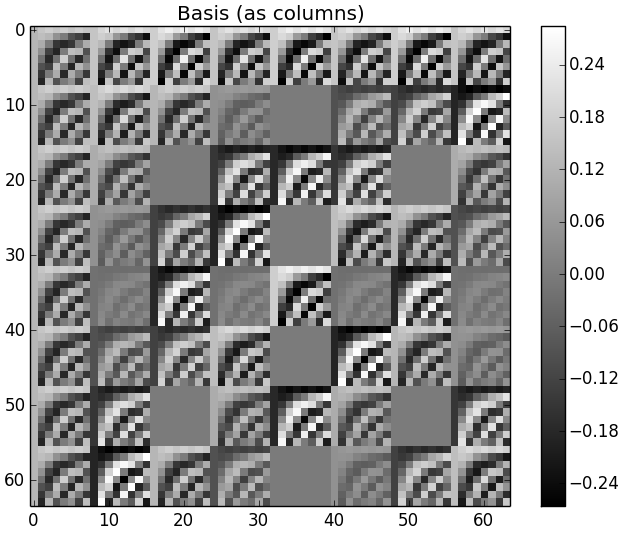
\includegraphics[width=1.1  in]{figs/Basis.png}
%\includegraphics[width=1.1  in]{figs/Ahat_FastICA_M640_K1_noise0_0001.png}
%\includegraphics[width=1.1  in]{figs/Ahat_FastICA_M640_K1_noise0_2042.png}
%\includegraphics[width=1.1  in]{figs/Ahat_FastICA_M640_K1_noise0_4083.png}
%\includegraphics[width=1.1  in]{figs/Ahat_FastICA_M640_K1_noise1_0205.png}
%\includegraphics[width=1.1  in]{figs/Ahat_FastICA_M640_K1_noise2_0409.png}
%\includegraphics[width=1.1  in]{figs/Ahat_FastICA_M640_K1_noise5_1021.png}
%\caption{BPD}
%\end{center}
%\end{figure*}
%







Such conditions for the \emph{identifiability} of the parameters underlying SCA were first investigated for the case $\mathbf{y}_i = A\mathbf{a}_i$ by Georgiev et. al. \cite{Georgiev05} and subsequently by Aharon et. al. \cite{Aharon06}. The most general conditions to date have recently been proven by Hillar and Sommer [cite], who provide deterministic and probabilistic guarantees for the identifiability of the model parameters contained in $A$ and the $\mathbf{a}_i$. We refine their proofs to take into account the possibility of noise contaminating the measurements (or inadequacy of the model) and to require a significantly reduced number of samples. These \emph{robust} identifiability conditions describe when the true model parameters can be uniquely determined in the sense of Definition \ref{Uniqueness}. Moreover, we provide guarantees for unique recovery of $A$ and the $\mathbf{a}_i$ when only an upper bound on the number of sources is known. Our conditions are derived from the underlying geometry of the dictionary learning problem, hence they apply regardless of which algorithm is used to solve \eqref{DictionaryLearning}. Table \ref{results} gives a summary of our results.

\begin{table}\label{results}
\begin{center}
$\begin{array}{c|cc} \text{Dataset } Y = \{A\mathbf{a}_1 + \mathbf{\eta}_1, \ldots,A\mathbf{a}_N + \mathbf{\eta}_N,\} \text{ with $k$-sparse } \mathbf{a}_i \in \mathbb R^m \text{ chosen:}   & \text{Total sufficient samples } N \text{ for a unique recovery}  \\\hline 
\text{in general position with $k{m \choose k}$ from each support set in $\mathcal{T}$, independent of $A$ satisfying spark condition (\ref{SparkCondition})}  & mk{m \choose k} \\\hline     
 \text{$k+1$ chosen "randomly" from each support set in $\mathcal{T}$, given matrix $A$ satisfying spark condition (\ref{SparkCondition})}  & m(k+1) \ \ \text{(with probability one)} \\\hline 
\text{$k+1$ chosen "randomly" from each support set in $\mathcal{T}$, independent of $A \notin Z$ 
}  & m(k+1) \ \ \text{(with probability one)} \\\hline 
\text{"randomly" from each support set in $\mathcal{T}$, given matrix $A$ satisfying spark condition (\ref{SparkCondition})}  & m(k+1)\beta^{-1}\ \ \text{(with probability $1-\beta$)} \\\hline 
\end{array}$
\end{center}
\caption{The number of subsamples sufficient for $Y = \{\mathbf{y}_1, \ldots,\mathbf{y}_N\}$ to have a unique sparse coding.}
\label{table_N}
\vspace{-.3 in}
\end{table}

Before stating our first theorem, it is instructive to first consider the simpler case where we wish to identify the sources $\mathbf{a}_i$ from the noiseless mixture $\mathbf{y}_i = A\mathbf{a}_i$ when $A$ is already known. Evidently, $A$ must satisfy the following \emph{spark condition}
\begin{align}\label{SparkCondition}
A\mathbf{a}_1 = A\mathbf{a}_2 \implies \mathbf{a}_1 = \mathbf{a}_2 \indent \text{for all $k$-sparse } \mathbf{a}_1, \mathbf{a}_2 \in \mathbb{R}^m
\end{align}
%
for such recovery to be possible. This condition ensures that distinct sparse sources are necessarily distinguishable in their measurements. As it turns out, this is also enough to guarantee uniqueness in the case where we don't know $A$ a priori, as our main result states:

%=== STATEMENT OF DETERMINISTIC UNIQUENESS THEOREM ===%

\begin{theorem}\label{DeterministicUniquenessTheorem}
Given positive integers $n, m$ and $k < m$, there exist $N =  mk{m \choose k}$ $k$-sparse vectors $\mathbf{a}_1, \ldots, \mathbf{a}_N \in \mathbb{R}^m$ with the following property: every matrix $A \in \mathbb{R}^{n \times m}$ satisfying spark condition \eqref{SparkCondition} has associated with it some $\varepsilon_0 > 0$ such that every dataset $Y = \{ \mathbf{y}_1, ..., \mathbf{y}_N \}$ for which $\| \mathbf{y}_i - A\mathbf{a}_i \|_2 \leq \varepsilon_0$ for all $i = 1, \ldots, N$ has a unique $k$-sparse coding. 
\end{theorem}

In fact, there are many such sets of deterministically produced $\mathbf{a}_i$; we give a parametrized family in Section \ref{DUT}. Note that if we restrict our attention to noiseless datasets of the form $\mathbf{y}_i = A\mathbf{a}_i$ then we recover Theorem 1 in [HS11] with an added improvement on $N$, the number of samples required to guarantee uniqueness. In fact, all of the theorems and corollaries in [HS11] are corollaries of our theorems. Our proofs are generalizations of the basic framework laid out in their paper.

The particular value of $\varepsilon_0$ associated to each $A$ satisfying \eqref{SparkCondition} and the values of $C$ and $C'$ alluded to in Definition \ref{Uniqueness} can be explicitly calculated from certain properties of $A$ and the $\mathbf{a}_i$ which we now define. A simple compactness argument can be made to show that any matrix satisfying \eqref{SparkCondition} must also satisfy
\begin{align}\label{RIP}
\|A\mathbf{a}_1 - A\mathbf{a}_2 \|_2 \geq  \alpha \|\mathbf{a}_1 - \mathbf{a}_2\|_2 \indent \text{ for all $k$-sparse } \mathbf{a}_1, \mathbf{a}_2 \in \mathbb{R}^m
\end{align}
%
for some $\alpha \in (0,1]$. We can equally well say that $\|A\mathbf{x}\| \geq \alpha\|\mathbf{x}\|$ for all $2k$-sparse $\mathbf{x} \in \mathbb{R}^{n \times m}$, or every $n \times \min(m,2k)$ submatrix of $A$ has lower bound $\alpha$. Since $A$ is a real matrix, it also has bounded norm and hence \eqref{RIP} is equivalent to the \emph{restricted isometry property} \cite{CandesTao05} familiar from work in the field of compressed sensing.

It can be shown (see the Appendix) that \eqref{SparkCondition} implies the existence of a nonzero \emph{Friedrichs angle} $\theta_F \in (0,\frac{\pi}{2}]$ (also known as the minimal Jordan angle) between all pairs of subspaces spanned by the columns of $A$ of dimensionality less than or equal to $k$. For completeness we state the definition of $\theta_F$ here:

\begin{definition}\label{FriedrichsDefinition}
The \emph{Friedrichs angle} $\theta_F(V,W) \in [0,\frac{\pi}{2}]$ between subspaces $V,W \subseteq \mathbb{R}^m$ is the minimal angle formed between unit vectors in $V \cap (V \cap W)^\perp$ and $W \cap (W \cap V)^\perp$, that is
\begin{align}
\cos\left[\theta_F(V,W)\right] := \max\left\{ \frac{ \langle v, w \rangle }{\|v\|\|w\|}: v \in V \cap (V \cap W)^\perp, w \in W \cap (V \cap W)^\perp \right\}
\end{align}
\end{definition}

We define the following quantity for notational convenience:

\begin{definition}\label{SpecialSupportSet}
Given $A \in \mathbb{R}^{n \times m}$ and $k < m$, let $\mathcal{T}$ be the set of all $S_i := \{i, \ldots, (i + (k-1) \} \;\bmod\; m$ for $i = 0, \ldots, m-1$. We define the quantity
\begin{align}\label{rho}
\phi_k(A) := \min_{ i_1 \neq \ldots \neq i_{\ell} \in [m]} \left\{ 1 - c(\text{Span}\{A_{S_{i_1}}\}, \ldots, \text{Span}\{A_{S_{i_\ell}}\}) \right\},
\end{align}
where for any sequence $V_1, \ldots, V_p$ of closed subspaces of $\mathbb{R}^m$,
\begin{align}
c(V_1, \ldots, V_p) := \left[1 - \prod_{i=1}^{p-1} \left(1 - \cos^2\left[ \theta_F(V_i, \cap_{j=i+1}^p V_j) \right] \right) \right]^{1/2} 
\end{align}
%
and we set $\phi_1(A) := 1$.
\end{definition}

We now state the specifics of Theorem \ref{DeterministicUniquenessTheorem} in terms of these quantities.

%=== SPECIFICS OF DETERMINISTIC THEOREM ===%

\begin{remark}[Theorem \ref{DeterministicUniquenessTheorem} cont'd]
Specifically, the $\mathbf{a}_i$ are constructed so that any $k$ of them are linearly independent. In particular, any $k$ vectors $\mathbf{a}_i$ sharing the same support satisfy
\begin{align}\label{DataSpread}
\|\sum_{j = 1}^k c_j \mathbf{a}_{i_j}\|_2 \geq \sigma \|c\|_2 \indent \text{for all } c = (c_1, ..., c_k) \in \mathbb{R}^k.
\end{align}
%
for some $\sigma > 0$. If $A$ has unit norm columns and satisfies spark condition \eqref{SparkCondition} with all $n \times k$ and $n \times \min(m,2k)$ submatrices of $A$ having lower bounds $\alpha_k$ and $\alpha_{2k}$, respectively, then for any matrix $B \in \mathbb{R}^{n \times m}$ and $k$-sparse $\mathbf{b}_i \in \mathbb{R}^m$ for which $\|\mathbf{y}_i - B\mathbf{b}_i\| \leq \varepsilon$ with $\varepsilon < \frac{\alpha^2\sigma\phi_k(A)}{(2k)^{2/3}}$ we have
\begin{align}
\|A - BPD\|_1 \leq \frac{2\varepsilon k^{2/3}\sqrt{m} }{\alpha_k\sigma \phi_k(A)}
\end{align}
%
for some permutation matrix $P \in \mathbb{R}^{m \times m}$ and invertible diagonal matrix $D \in \mathbb{R}^{m \times m}$. Moreover, 
\begin{align}\label{b_PDa}
\|\mathbf{b}_i - PD\mathbf{a}_i\|_1 \leq \frac{\varepsilon}{\alpha_{2k}\|D\|_2}  \left( 1 + \frac{2 k^{2/3}}{\alpha_k\sigma \phi_k(A)}\|D^{-1}P^{-1}\mathbf{b}_i\|_1 \right).
\end{align}
\end{remark}

Our next result exploits randomness to give a different construction requiring fewer samples. Fix a matrix $A$ satisfying spark condition \eqref{SparkCondition} and a small $\beta > 0$. There is a simple random drawing procedure (Definition \ref{RandomDraw}) for generating $N = \beta^{-1}m(k+1)$ $k$-sparse vectors $\mathbf{a}_1, \ldots, \mathbf{a}_N$ such that $Y = \{A\mathbf{a}_1 + \mathbf{\eta}_1, \ldots, A\mathbf{a}_N + \mathbf{\eta}_N\}$ has a unique sparse coding (with probability at least $1 - \beta$), provided $\|\mathbf{\eta}_i\|$ is bounded by a small enough constant. In particular, sparse matrix factorization of sparsely coded data is typically unique for a number of samples linear in the dimensionality and sparsity level of the sparse codes, provided their supports are distributed enough over those contained in a special support set (specifically, $\mathcal{T}$ from Definition \ref{SpecialSupportSet}).

A subtle difference between these two results is that $\mathbf{a}_1, \ldots, \mathbf{a}_N$ in Theorem \ref{DeterministicUniquenessTheorem} are independent of the generation matrix $A$. The following statement is the best we are able to do in this direction using random methods. With probability one, a random draw of $(k+1)$ $k$-sparse $\mathbf{a}_i$ from each of the $m$ support sets in $\mathcal{T}$ satisfies the following property. There is a set of matrices $Z \in \mathbb{R}^{n \times m}$ with Lebesgue measure zero such that if $A \notin Z$, then there exists some $\varepsilon_0$ small enough such that $Y = \{A\mathbf{a}_1 + \mathbf{\eta}_1, \ldots, A\mathbf{a}_N + \mathbf{\eta}_N\}$ for $\|\mathbf{\eta}_i\| \leq \varepsilon_0$ has a unique sparse coding.

It is important for us to note how these theorems of ours fit in with others comprising the field of \emph{theoretical dictionary learning}. While a collection of greedy optimization algorithms have been proposed for solving \eqref{DictionaryLearning}, as yet there exist no global convergence guarantees for these techniques. Local identifiability analyses have demonstrated that the global minimum is a local minimum of cost functions of L0 and L1 cost functions, (local) convergence guarantees of greedy and convex algorithms. A most welcome corollary to our theorems is a closed form expression for checking when any dictionary learning algorithm has converged to a global minimum of \eqref{DictionaryLearning} by asserting whether or not the reconstruction error of the proposed solution is indeed small enough. 

It is also informative to elaborate on the relationship of our results to the field of compressive sensing. [ref?] CS theory provides conditions under which it is possible to recover data vectors $\mathbf{x}$ with sparse structure after they have been linearly subsampled as $\mathbf{y} = \Phi \mathbf{a}$ by a known compression matrix $\Phi$. The sparsity usually enforced is that the vectors $\mathbf{x}$ can be expressed as $\mathbf{x} = \Psi\mathbf{a}$ using a known dictionary matrix $\Psi$ and $m$-dimensional vectors $\mathbf{a}$ with at most $k < m$ nonzero entries. Such vectors $\mathbf{a}$ are called $k$-\emph{sparse}. A necessary condition for the unique recovery of $\mathbf{a}$ given $\mathbf{y}$ is that the generation matrix $A = \Phi\Psi$ satisfy the spark condition \eqref{SparkCondition}. Otherwise, different sparse sources would be indistinguishable in the compressed space. Provided the dimension $n$ of $\mathbf{y}$ satisfies
\begin{align}\label{CScondition}
n \geq Ck\log\left(\frac{m}{k}\right),
\end{align}
%
the theory guarantees that with high probability a randomly generated $\Phi$ will yield an $A$ satisfying \eqref{SparkCondition}. In contrast, the goal of SCA is to recover both the code vectors \emph{and} the generation matrix from measurements. We show that the same uniqueness conditions required by CS also guarantee uniqueness in SCA given enough samples distributed over suitable supports.

The organization of this paper is as follows.in Section \ref{DUT} we state our main tool from combinatorial matrix theory and then derive from it Theorem \ref{DeterministicUniquenessTheorem}. We next provide precise statements in Section \ref{PUT} of our randomized theorems and then prove them in Section \ref{PUTproof}. In Section (??) we describe how to extend the theorems in the previous sections to the case where we have only an upper bound on the number of sparse components. The final section is a discussion. An appendix contains the proof of Lemma \ref{MainLemma} as well as some auxiliary proofs. 

Have the cool small dimensional example here. Data in $3D$-space coded by planes. $n=3, k=2$. 

Implication: overcomplete dimensionality of any dataset with respect to $\varepsilon$. If you coded very well some data sparsely then you can do a check and if that check holds up then anyone else who codes the data sparsely too has learned the same dictionary. 
 
%============================================
% PROOF OF DETERMINISTIC UNIQUENESS THEOREM
%============================================

\section{Deterministic Uniqueness Theorem}\label{DUT}

In what follows, we will use the notation $[m]$ for the set $\{1, ..., m\}$, and ${[m] \choose k}$ for the set of subsets of $[m]$ of cardinality $k$. Also, recall that $\text{Span}\{\mathbf{v}_1, \ldots, \mathbf{v}_\ell\}$ for real vectors $\mathbf{v}_1, \ldots, \mathbf{v}_\ell$ is the vector space consisting of their $\mathbb{R}$-linear span:
%
\[ \text{Span}\{\mathbf{v}_1, \ldots, \mathbf{v}_\ell\} = \left\{ \sum_{i=1}^\ell t_i\mathbf{v}_i : t_1, \ldots, t_\ell \in \mathbb{R}\right\}. \]
%
Finally, for a subset $S \subseteq [m]$ and matrix $A$ with columns $\{A_1,...,A_m\}$ we define
%
\[ \text{Span}\{A_S\} = \text{Span}\{A_s: s \in S\}. \]

%======== CASE K = 1 ============

Before proving Theorem \ref{DeterministicUniquenessTheorem} in full generality it is illustrative to consider the case when $k=1$. In this simple case, we only need $N = m$ samples to guarantee uniqueness. Set $\mathbf{a}_i = \mathbf{e}_i$ $(i = 1, \ldots, m)$ to be the standard basis vectors in $\mathbb{R}^m$ and suppose that our data $Y = \{\mathbf{y}_1, \ldots, \mathbf{y}_N\}$ satisfies $\|\mathbf{y}_i - A\mathbf{a}_i\|_2 \leq \varepsilon$ for all $i \in [m]$ for some $A \in \mathbb{R}^{n \times m}$ with unit norm columns satisfying \eqref{RIP} and that $\varepsilon < \frac{\alpha}{2\sqrt{2}}$. Assuming that $\|\mathbf{y}_i - B\mathbf{b}_i\|_2 \leq \varepsilon$ for all $i \in [m]$ for some alternate $B \in \mathbb{R}^{n \times m}$ and 1-sparse $\mathbf{b}_i \in \mathbb{R}^m$, then by the triangle inequality we have $\|A\mathbf{a}_i - B\mathbf{b}_i\| \leq 2\varepsilon$ for all $i \in [m]$. Since the $\mathbf{b}_i$ are 1-sparse, there must exist $c_1, \ldots, c_m \in \mathbb{R}$ such that 
\begin{align}\label{1D}
\|A\mathbf{e}_i - c_iB\mathbf{e}_{\pi(i)}\|_2 \leq 2\varepsilon \indent \text{for all} \indent i \in [m].
\end{align}
for some map $\pi: [m] \to [m]$. 
Note that if $c_i = 0$ for some $i$, then $\|A\mathbf{e}_i\| < 1$ (since $\alpha \leq 1$), contradicting the fact that $A$ has unit norm columns. We will now show that $\pi$ is necessarily injective (and thus defines a permutation). Suppose that $\pi(i) = \pi(j) = \ell$ for some $i \neq j$ and $\ell \in [m]$. Then $\|A\mathbf{e}_i - c_iB\mathbf{e}_{\ell}\|_2  \leq 2\varepsilon$ and $\|A\mathbf{e}_j - c_jB\mathbf{e}_{\ell}\|_2 \leq 2\varepsilon$. Summing and scaling these two inequalities by $|c_j|$ and $|c_i|$, respectively, we apply the triangle inequality and then \eqref{RIP} to yield
\begin{align*}
(|c_i| + |c_j|) 2\varepsilon
&\geq |c_j|\|A\mathbf{e}_i - c_iB\mathbf{e}_{\ell}\|_2 + |c_i|\|c_jB\mathbf{e}_{\ell} - A\mathbf{e}_j\|_2 \\
&\geq \|c_jAe_i + c_iAe_j\|_2 \\
&\geq \alpha\|c_je_i + c_ie_j\|_2
\end{align*}
%
which is in contradiction with the fact that $\|x\|_1 \leq \sqrt{2}\|x\|_2$ for all $x \in \mathbb{R}^2$ and $\varepsilon < \frac{\alpha}{2\sqrt{2}}$. Hence, $\pi$ is injective. Letting $P$ and $D$ denote the following permutation and diagonal matrices, respectively:
\begin{equation}\label{PandD}
P = \left( \mathbf{e}_{\pi(1)} \cdots \mathbf{e}_{\pi(m)}\right), \ \ D = \left(\begin{array}{ccc}c_1 & \cdots & 0 \\\vdots & \ddots & \vdots \\0 & \cdots & c_m\end{array}\right),
\end{equation}
%
we see that \eqref{1D} becomes $\|(A - BPD)\mathbf{e}_i\|_2 \leq 2\varepsilon$ for all $i \in [m]$ and it follows that $\|A-BPD\|_1 \leq 2\sqrt{m}\varepsilon$.

% ========  A = BPD  ----> b = PDa  ====================

Note that the identity $\|(A - BPD)\mathbf{e}_i\|_2 \leq C\varepsilon$ for some $C > 0$ together with \eqref{RIP} already implies in general the recovery result $\|\mathbf{b}_i - PD\mathbf{a}_i\|_1 \leq C'\varepsilon$ for $C' > 0$ for all $i \in [m]$. This follows since for any $k$-sparse vector $\mathbf{a}_i = \sum_{\ell=1}^{k} c_\ell \mathbf{e}_{i_\ell}$ we have by the triangle inequality that $\|(A-BPD)v\| \leq \sum_{\ell=1}^{k}|c_\ell| \|(A-BPD)\mathbf{e}_{i_\ell}\|$, hence
\begin{align*}
\|(A - BPD)D^{-1}P^{-1}\mathbf{b}_i\| \leq \|D^{-1}P^{-1}\mathbf{b}_i\|_1C\varepsilon.
\end{align*}
%
It then follows by the triangle inequality and \eqref{RIP} that
\begin{align*}
\alpha \|D^{-1}P^{-1}\mathbf{b}_i - \mathbf{a}_i\| &\leq \|A(D^{-1}P^{-1}\mathbf{b}_i - \mathbf{a}_i)\| \\
&\leq \| AD^{-1}P^{-1}\mathbf{b}_i - B\mathbf{b}_i\| + \|B\mathbf{b}_i - \mathbf{y}_i\| + \|\mathbf{y}_i - A\mathbf{a}_i\| \\
&\leq  \varepsilon  \left( 2 + C\|D^{-1}P^{-1}\mathbf{b}_i\|_1 \right).
\end{align*}

Hence,
\begin{align}
\|\mathbf{b}_i - PD\mathbf{a}_i\| \leq  \frac{\varepsilon}{\alpha\|D\|_2}\left( 2 + C\|D^{-1}P^{-1}\mathbf{b}_i\|_1 \right)
\end{align}

% ========== DEFINITIONS FOR MAIN LEMMA (K>1) ================

Unfortunately, the proof for larger $k$ is more challenging since in general it is nontrivial to produce $P$ and $D$ as in \eqref{PandD}. For this, we require an additional result in combinatorial linear algebra. We make one more definition before stating the relevant lemma.  

\begin{definition}
Let $V, W$ be subspaces of $\mathbb{R}^m$ and let $d(v,W) := \inf\{\|v-w\|_2: w \in W\} = \|v - \Pi_W v\|$ where $\Pi_W$ is the orthogonal projection operator onto subspace $W$. The \emph{gap} metric $\Theta$ on subspaces of $\mathbb{R}^{m}$ is [see Theory of Linear Operators in a Hilbert Space p. 69 who cites first reference]
\begin{equation}\label{SubspaceMetric}
\Theta(V,W) := \max\left( \sup_{\substack{v \in V \\ \|v\| = 1}} d(v,W), \sup_{\substack{w \in W \\ \|w\| = 1}} d(w,V) \right).
\end{equation}
\end{definition}
%
In our proof we will make use of the following useful facts:
\begin{equation}\label{SubspaceMetricSameDim}
\dim(W) = \dim(V) \implies \sup_{\substack{v \in V \\ \|v\| = 1}}  d(v,W)  = \sup_{\substack{w \in W \\ \|w\| = 1}} d(w,V),
\end{equation}
%
a proof of which can be found in \cite{Morris10} (Lemma 3.3) and
\begin{equation}\label{MinDim}
d(v,W) < \|v\|_2 \indent \forall v \in V \implies \dim(V) \leq \dim(W).
\end{equation}

A quick proof of \eqref{MinDim} is as follows. If $\dim(V) > \dim(W)$ then there exists some $v' \in V \cap W^\perp$ and by Pythagoras' Theorem, $\|v' - w\|_2^2 = \|v'\|_2^2 + \|w\|_2^2 \geq \|v\|_2^2$ for all $w \in W$. This is in contradiction with the LHS of \eqref{MinDim}, which states that for all $v \in V$ there exists some $w \in W$ such that $\|v - w\|_2 < \|v\|_2$.

We now state our main result from combinatorial matrix theory.

%===========          MAIN LEMMA (K > 1)             =================

\begin{lemma}[Main Lemma]\label{MainLemma}
Fix positive integers $n, m$ and $k < m$. Let $A, B \in \mathbb{R}^{n \times m}$ and suppose that $A$ has unit norm columns, satisfies spark condition \eqref{SparkCondition}, and every $n \times \max(2,k)$ submatrix of $A$ has lower bound $\alpha \in (0,1]$. Let $\mathcal{T}$ be the set of all $S_i := \{i, \ldots, (i + (k-1) \} \;\bmod\; m$ for $i = 0, \ldots, m-1$. If there exists a map $\pi: \mathcal{T} \to {[m] \choose k}$ and some $\Delta < \frac{\alpha}{\sqrt{2}}$ such that 
\begin{equation}\label{GapUpperBound}
\Theta(\text{Span}\{A_{S_i}\}, \text{Span}\{B_{\pi(S_i)}\}) \leq \frac{ \phi_k(A) }{k} \Delta \indent \text{for all} \indent i \in \{0, \ldots, m-1\}
\end{equation}
%
then there exist a permutation matrix $P \in \mathbb{R}^{m \times m}$ and a diagonal matrix $D \in \mathbb{R}^{m \times m}$ such that
\begin{align}
\|A - BPD\|_1 \leq \sqrt{m}\Delta \indent \text{for all} \indent i \in [m].
\end{align}
\textbf{[Is there a better norm to use here?]}
\end{lemma}

We defer the proof of this lemma to the Appendix. 

%========          PROOF OF THEOREM 1        ============

\begin{proof}[Proof of Theorem \ref{DeterministicUniquenessTheorem}]
First, we produce a set of $N = mk{m \choose k}$ vectors in $\mathbb{R}^k$ in general linear position (i.e. any set of $k$ of them are linearly independent). Specifically, let $\gamma_1, ..., \gamma_N$ be any distinct numbers. Then the columns of the $k \times N$ matrix $V = (\sigma^i_j)^{k,N}_{i,j=1}$ are in general linear position (since the $\sigma_j$ are distinct, any $k \times k$ "Vandermonde" sub-determinant is nonzero). Next, form the $k$-sparse vectors $\mathbf{a}_1, \ldots, \mathbf{a}_N \in \mathbb{R}^m$ with supports $S_j = \{j, \ldots, (j + k-1)\;\bmod\; m \}$ for $j \in [m]$ (partitioning the $a_i$ evenly among these supports, i.e. for each support $S_j$ there are $k{m \choose k}$ vectors $a_i$ with that support) by setting the nonzero values of vector $\mathbf{a}_i$ to be those contained in the $i$th column of $V$. Note that by construction every $k$ vectors $a_i$ are linearly independent. 

We will show how the existence of these $\mathbf{a}_i$ proves the theorem. First, we will show that they satisfy property \eqref{DataSpread}. Consider the compact set $\mathcal{C} = \{c \in \mathbb{R}^k: \|c\|_2 = 1\}$ and the continuous map
\begin{align*}
\phi: \mathcal{C} &\to \mathbb{R} \\
(c_1, ..., c_k) &\mapsto \|\sum_{j = 1}^k c_j \mathbf{a}_{i_j}\|_2.
\end{align*}

By general linear position of the $\mathbf{a}_i$, we know that $0 \notin \phi(\mathcal{C})$. Since $\mathcal{C}$ is compact, we have by continuity of $\phi$ that $\phi(\mathcal{C})$ is also compact; hence it is closed and bounded. Therefore $0$ can't be a limit point of $\phi(\mathcal{C})$ and there must be some $\sigma > 0$ such that the neighbourhood $\{x: x < \sigma\} \subseteq \mathbb{R} \setminus \phi(\mathcal{C})$. Hence $\phi(c) \geq \sigma$ for all $c \in \mathcal{C}$. The property \eqref{DataSpread} follows by the association $c \mapsto \frac{c}{\|c\|_2}$ and the fact that there are only finitely many subsets of $k$ vectors $\mathbf{a}_i$ (actually, for our purposes we need only consider those subsets of $k$ vectors $\mathbf{a}_i$ having the same support), hence there is some minimal $\delta$ satisfying \eqref{DataSpread} for all of them. (We refer the reader to the Appendix for a lower bound on $\sigma$ given as a function of $k$ and the sequence $\gamma_1, \ldots, \gamma_N$ used to generate the $a_i$.)

Now suppose that $Y = \{\mathbf{y}_1, \ldots, \mathbf{y}_N\}$ is a dataset for which for all $i \in \{1, \ldots, N\}$ we have $\|\mathbf{y}_i - A\mathbf{a}_i\| \leq \varepsilon$ for some $\varepsilon > 0$ and $A \in \mathbb{R}^{n \times m}$ with all $n \times k$ submatrices of $A$ having lower bound $\alpha$. Suppose further that for some alternate $B \in \mathbb{R}^{n \times m}$ there exist $k$-sparse $\mathbf{b}_i \in \mathbb{R}^m$ for which $\|\mathbf{y}_i - B\mathbf{b}_i\| \leq \varepsilon$ for all $i \in \{1, \ldots, N\}$. Since there are $k{m \choose k}$ vectors $\mathbf{a}_i$ with a given support $S$, the pigeon-hole principle implies that there are at least $k$ vectors $\mathbf{y}_i$ such that $\|\mathbf{y}_i - A\mathbf{a}_i\| \leq \varepsilon$ for these $\mathbf{a}_i$ and also $\|\mathbf{y}_i - B\mathbf{b}_i\| \leq \varepsilon$ for $\mathbf{b}_i$ all sharing the same support $S' \in {[m] \choose k}$. \textbf{[Do we really need this many samples per support? Consider the information gained by noting that we have vectors distributed over multiple supports and that $A$ satisfies the spark condition.]} Let $\mathcal{Y}$ be a set of $k$ such vectors $\mathbf{y}_i$ which we will index by $\mathcal{I}$, i.e. $\mathcal{Y} = \{\mathbf{y}_i: i \in \mathcal{I}\}$.

It follows from the general linear position of the $\mathbf{a}_i$ and the fact that every $k$ columns of $A$ are linearly independent that the set $\{A\mathbf{a}_i: i \in \mathcal{I}\}$ is a basis for $\text{Span}\{A_S\}$. Hence, fixing $\mathbf{z} \in \text{Span}\{A_S\}$, there exists a unique set of $c_i \in \mathbb{R}$ (for notational convenience we index these $c_i$ with $\mathcal{I}$ as well) such that $\mathbf{z} = \sum_{i \in \mathcal{I}} c_iA\mathbf{a}_i$. Letting $\mathbf{y} = \sum_{i \in \mathcal{I}} c_i\mathbf{y}_i  \in \text{Span}\{\mathcal{Y}\}$, we have by the triangle inequality that
\begin{align}\label{4}
\|\mathbf{z} - \mathbf{y}\|_2 = \| \sum_{i \in \mathcal{I}} c_i A \mathbf{a}_i -  \sum_{i \in \mathcal{I}} c_i \mathbf{y}_i \|_2 \leq \sum_{i \in \mathcal{I}} \| c_i (A\mathbf{a}_i - \mathbf{y}_i) \|_2 = \sum_{i \in \mathcal{I}} |c_i| \| A\mathbf{a}_i - \mathbf{y}_i \|_2 \leq \varepsilon \sum_{i \in \mathcal{I}} |c_i|.
\end{align}

The alternate factorization for the $\mathbf{y}_i$ implies (by a manipulation identical to that of \eqref{4}) that for $\mathbf{z}' = \sum_{i \in \mathcal{I}} c_i B\mathbf{b}_i \in \text{Span}\{B_{S'}\}$ we have $\|\mathbf{y} - \mathbf{z}'\|_2 \leq \varepsilon \sum_{i \in \mathcal{I}} |c_i|$ as well. It follows again by the triangle inequality that
\begin{align}\label{dist}
\|\mathbf{z} - \mathbf{z}'\|_2 \leq \|\mathbf{z} - \mathbf{y}\|_2 + \|\mathbf{y} - \mathbf{z}'\|_2 = 2 \varepsilon \sum_{i \in \mathcal{I}} |c_i|.
\end{align}

Since $\text{supp}(\mathbf{a}_i) = S$ for all $i \in \mathcal{I}$ and $A$ has $k$-sparse restricted lower bound $\alpha$, we have 
\begin{align}\label{len}
\|\mathbf{z}\|_2 = \|\sum_{i \in \mathcal{I}}^k c_i A \mathbf{a}_i\|_2 
= \|A (\sum_{i \in \mathcal{I}} c_i \mathbf{a}_i) \|_2 
\geq \alpha \|\sum_{i \in \mathcal{I}}^k c_i \mathbf{a}_i\|_2 
\geq \frac{\alpha\sigma}{\sqrt{k}}\sum_{i \in \mathcal{I}}^k |c_i|,
\end{align}
%
where for the last inequality we have applied the property \eqref{DataSpread}, noting that $\sqrt{k}\|c\|_2 \geq \|c\|_1$ for all $c \in \mathbb{R}^k$. Combining \eqref{dist} and \eqref{len}, we see that for all $\mathbf{z} \in \text{Span}\{A_S\}$ there exists some $\mathbf{z}' \in \text{Span}\{B_{S'}\}$ such that $\|\mathbf{z} - \mathbf{z}'\|_2 \leq \frac{ 2 \varepsilon \sqrt{k}}{ \alpha \sigma } \|\mathbf{z}\|_2$. It follows that $d(\mathbf{z}, \text{Span}\{B_{S'}\}) \leq \frac{ 2 \varepsilon \sqrt{k} }{ \alpha \sigma }$ for all unit vectors $\mathbf{z} \in \text{Span}\{A_S\}$. Hence,
\begin{align}\label{ABSubspaceDistance}
\sup_{ \substack{ \mathbf{z} \in \text{Span}\{A_{S}\} \\ \|\mathbf{z}\| = 1} } d(\mathbf{z}, \text{Span}\{B_{S'}\}) \leq \frac{ 2 \varepsilon \sqrt{k} }{ \alpha \sigma }.
\end{align}

If $\varepsilon < \frac{\alpha\sigma}{2\sqrt{k}}$, we have that $\dim(\text{Span}\{B_{S'}\}) \geq \dim(\text{Span}\{A_S\}) = k$ by \eqref{MinDim} and the fact that every $k$ columns of $A$ are linearly independent . In fact, since $|S'| = k$, we have $\dim(\text{Span}\{B_{S'}\}) = \dim(\text{Span}\{A_S\})$. Recalling \eqref{SubspaceMetricSameDim},  we see the association $S \mapsto S'$ thus defines a map $\pi: \{S_1, \ldots, S_m\} \to {[m] \choose k}$ satisfying $\Theta(\text{Span}\{A_S\}, \text{Span}\{\mathcal{B_{\pi(S)}}\}) \leq \frac{ 2 \varepsilon \sqrt{k} }{ \alpha \delta }$.

If $\varepsilon < \frac{\alpha^2\sigma\phi_k(A)}{(2k)^{2/3}}$, we then indeed have $\varepsilon < \frac{\alpha\sigma}{2\sqrt{k}}$ (since $\alpha \leq 1$, $\phi_k(A) \leq 1$ and $k \geq 1$) so that 
\begin{align}\label{SubspaceDistanceUpperBound}
\Theta(\text{Span}\{A_{S_i}\}, \text{Span}\{\mathcal{B}_{\pi(S_i)}\}) \leq \frac{\phi_k(A)}{k}\Delta
\indent \text{for all} \indent i = 0, \ldots, m-1,
\end{align}
%
where $\Delta = \frac{2k^{2/3}\varepsilon}{\alpha\sigma\phi_k(A)} < \frac{\alpha}{\sqrt{2}}$. Moreover, it follows by Lemma \ref{MainLemma} that there exists a permutation matrix $P \in \mathbb{R}^{m \times m}$ and a diagonal matrix $D \in \mathbb{R}^{m \times m}$ such that for all $i \in \{1, \ldots, m\}$,
$\|A - BPD\|_1 \leq C\varepsilon$ for $C = \frac{2k^{2/3}\sqrt{m}}{\alpha\sigma\phi_k(A)}$.
\end{proof}

\begin{corollary}

\end{corollary}

\begin{proof}

\end{proof}

%======================================
% STATEMENTS OF PROBABILISTIC THEOREMS
%======================================

\section{Statements of Probabilistic Theorems}\label{PUT}

We next give precise statements of our probabilistic versions of Theorem 1, all of which rely on the following construction.

\begin{definition}[Random Sparse Vectors]\label{RandomDraw}
Given the support set for its $k$ nonzero entries, a random draw of $\mathbf{a}$ is the $k$-sparse vector with support entries chosen uniformly from the interval $[0, 1] \subset \mathbb{R}$, independently. When a support set is not specified, a random draw is a choice of one support set uniformly from all of them in ${[m] \choose k}$ and then a random draw.
\end{definition}

\begin{definition}[Special Random Sparse Vectors]\label{SpecialRandomDraw}
Given the support set for its $k$ nonzero entries, a random draw of $\mathbf{a}$ is the $k$-sparse vector with support entries chosen uniformly from the interval $[0, 1] \subset \mathbb{R}$, independently. When a support set is not specified, a random draw is a choice of one support set uniformly from all $m$ of them in $\mathcal{T}$ and then a random draw.
\end{definition}

\begin{theorem}\label{Theorem2}
Fix positive integers $k < m$ and $n$, and a generation matrix $A \in \mathbb{R}^{n \times m}$ satisfying spark condition \eqref{SparkCondition}. If $(k+1)$ $k$-sparse $\mathbf{a}_i$ are randomly drawn from each support set in $\mathcal{T}$, then $Y = \{A\mathbf{a}_1 + \mathbf{\eta}_1, \ldots ,  A\mathbf{a}_N + \mathbf{\eta}_N \}$ for $\|\mathbf{\eta}_i\| \leq \varepsilon$ has a unique sparse coding with probability one, provided $\varepsilon$ is small enough.
\end{theorem}

The following is a direct application of this result, partially answering one of our questions from the introduction.

\begin{corollary}
Suppose $m, n$, and $k$ satisfy inequality \eqref{CScondition}. With probability one, a random \textbf{[insert footnote explaining 'random']} $n \times m$ generation matrix $A$ satisfies \eqref{SparkCondition}. Fixing   such an $A$, for $\varepsilon$ small enough we have with probability one that a dataset $Y = \{A\mathbf{a}_1 + \mathbf{\eta}_1, . . . , A\mathbf{a}_N + \mathbf{\eta}_1 \}$ for $\|\mathbf{\eta}_i\| \leq \varepsilon$ generated from $N = (k + 1)m$ $k$-sparse samples $\mathbf{a}_i$ uniquely prescribes $A$ and these sparse vectors $\mathbf{a}_i$ up to an approximate fixed permutation and scaling.
\end{corollary}

We now state our third theorem. Note that an \emph{algebraic set} is a solution to a finite set of polynomial equations. 

\begin{theorem}\label{Theorem3}
Fix positive integers $k < m$ and $n$. If $(k + 1)$ $k$-sparse $\mathbf{a}_i$ are randomly drawn from each support set in $\mathcal{T}$, then with probability one the following holds. There is an algebraic set $Z \subset \mathbb{R}^{n \times m}$ of Lebesgue measure zero with the following property: if $A \notin Z$ then there exists some $\varepsilon$ small enough such that $Y = \{A\mathbf{a}_1 + \mathbf{\eta}_1, . . . , A\mathbf{a}_N + \mathbf{\eta}_1 \}$ for $\|\mathbf{\eta}_i\| \leq \varepsilon$ has a unique sparse coding.
\end{theorem}

\begin{corollary}
Suppose $m, n$, and $k$ obey inequality \eqref{CScondition}. With probability one, a random draw of $N = (k + 1)m$ $k$-sparse samples $\mathbf{a}_i$ with supports in $\mathcal{T}$ satisfies: for almost every matrix $A$ there is some $\varepsilon$ small enough that gives $Y = \{A\mathbf{a}_1 + \mathbf{\eta}_1, . . . , A\mathbf{a}_N + \mathbf{\eta}_1 \}$ for $\|\mathbf{\eta}_i\| \leq \varepsilon$ a unique sparse coding.
\end{corollary}

%===================================
% PROOFS OF PROBABILISTIC THEOREMS
%===================================

\section{Proofs of Probabilistic Theorems}\label{PUTproof}

Definition \ref{RandomDraw}: can I bound the probability of drawing from one of the $m!$ special support sets without explicitly making that restriction?

The proofs of our probabilistic theorems follow the same logic as outlined in \cite{HS11}. 

\begin{lemma}
Fix $A \in \mathbb{R}^{n \times m}$ satisfying \eqref{RIP}. With probability one, if $k+1$ vectors $\mathbf{a}_i$ are such that $d(A\mathbf{a}_i,V) \leq (??)$ for some $k$-dimensional subspace $V \subset \mathbb{R}^m$ then all of the $k+1$ vectors $\mathbf{a}_i$ have the same supports.
\end{lemma}
\begin{proof}
We need only show that the $k+1$ vectors $A\mathbf{a}_i$ are linearly dependent; the rest follows by Lemma 3 from \cite{HS11}. Let these $k+1$ vectors $\mathbf{a}_i$ be indexed by $\mathcal{I}$ and let $W = \text{Span}\{A\mathbf{a}_{i \in \mathcal{I}}\}$. Then for all $w \in W$ we can write $w = \sum_{i \in \mathcal{I}} c_iA\mathbf{a}_i$ for some set of $c_i \in \mathbb{R}$. Letting $v = \sum_{i \in \mathcal{i}} c_iv_i$, it follows that
\[ \|w - v\| = \|\sum_{i \in \mathcal{I}} c_i A\mathbf{a}_i - \sum_{i \in \mathcal{I}} c_i v_i \| 
\leq \sum_{i \in \mathcal{I}} |c_i| \|A\mathbf{a}_i - v_i\| \leq 2\varepsilon \sum_{i \in \mathcal{I}}|c_i| \]

Need RHS less thatn $\|w\|$ to prove that $\dim(W) \leq \dim(V) = k$...
\end{proof}

\begin{proof}[Proof of Theorem \ref{Theorem2}]
Fix $n, m$ and $k < m$. Fix a real matrix $A \in \mathbb{R}^{n \times m}$ satisfying \eqref{SparkCondition} and suppose there is some $B \in \mathbb{R}^{n \times m}$ and $k$-sparse $\mathbf{b}_1, \ldots, \mathbf{b}_N$ such that $\|\mathbf{y}_i - B\mathbf{b}_i\| \leq \varepsilon$ for all $i \in \{1, \ldots, N\}$. Then by the triangle inequality we have $\|A\mathbf{a}_i - B\mathbf{b}_i\| \leq 2\varepsilon$ for all $i \in \{1, \ldots, N\}$. Given a support set $S \in {[m]\choose k}$, let $J(S) = \{j: \text{supp}(\mathbf{b}_j) \subseteq S\}$ and note that for all $j \in J(S)$ there exists some $v \in \text{Span}\{B_S\}$ such that $\|A\mathbf{a}_i - v\| \leq 2\varepsilon$. By Lemma (??), with probability one, either $|J(S)| \leq k$ for all $\mathbf{a}_j$ with $j \in J(S)$ have the same support.
\end{proof}



%===================================
% DIFFERENT CODING DIMENSIONS
%===================================

\section{Different coding dimensions}\label{mleqm}

In this section we address the issue of recovering $A \in \mathbb{R}^{n \times m}$ and the $\mathbf{a}_i \in \mathbb{R}^m$ when only an upper bound $m'$ on the number $m$ of sparse sources is known.

\begin{theorem}\label{DeterministicUniquenessTheorem2}
Given positive integers $n, m, m'$ and $k$ with $k < m \leq m'$, there exist $N =  mk{m' \choose k}$ $k$-sparse vectors $\mathbf{a}_1, \ldots, \mathbf{a}_N \in \mathbb{R}^m$ with the following property: if $Y = \{ \mathbf{y}_1, ..., \mathbf{y}_N \}$ is a dataset for which for some $A \in \mathbb{R}^{n \times m}$ satisfying spark condition \eqref{SparkCondition} we have $\| \mathbf{y}_i - A\mathbf{a}_i \|_2 \leq \varepsilon$ for all $i = 1, \ldots, N$, then any other matrix $A' \in \mathbb{R}^{n \times m'}$ also satisfying spark condition \eqref{SparkCondition} and for which there exist $k$-sparse $\mathbf{a'}_1, \ldots, \mathbf{a'}_N \in \mathbb{R}^{m'}$ such that $\| \mathbf{y}_i - A\mathbf{a'}_i \|_2 \leq \varepsilon$ for all $i = 1, \ldots, N$ necessarily satisfies $\|A - A'PD\| \leq C\varepsilon$ for some $C > 0$, permutation matrix $P \in \mathbb{R}^{m' \times m'}$ and diagonal matrix $D \in \mathbb{R}^{m' \times m}$, provided $\varepsilon$ is small enough. Moreover, this implies $\|\mathbf{b}_i - PD\mathbf{a}_i\|_1 \leq C'\varepsilon$ for some $C' > 0$.

Specifically, the $\mathbf{a}_i$ are constructed so that any $k$ of them are linearly independent. In particular, any set of $k$ vectors $\mathbf{a}_i$ that shate the same support satisfy \eqref{DataSpread} for some $\sigma > 0$. Letting $\Phi = \min(\phi_k(A), \phi_k(B))$, if all $n \times \max(2,k)$ and $n \times 2k$ submatrices of $A$ have lower bound $\alpha_k$ and $\alpha_{2k}$, respectively, then provided $\varepsilon < (2k)^{-2/3}\alpha_k^2\sigma \Phi$ we have
\begin{align}
\|A - BPD\|_1 \leq \frac{2\varepsilon k^{2/3}\sqrt{m} }{\alpha_k\sigma \Phi}
\end{align}
%
and 
\begin{align}\label{b_PDa}
\|\mathbf{b}_i - PD\mathbf{a}_i\|_1 \leq \frac{\varepsilon}{\alpha_{2k}\|D\|_2}  \left( 1 + \frac{2 k^{2/3}}{\alpha_k\sigma \phi_k(A)}\|D^TP^T\mathbf{b}_i\|_1 \right).
\end{align}
\end{theorem}

The proof of this adaptation of Theorem \ref{DeterministicUniquenessTheorem2} is very similar to the proof of Theorem \ref{DeterministicUniquenessTheorem}, the only difference being that now we establish a map $\pi: [m] \to [m']$ satisfying the requirements of Lemma \ref{MainLemma2}, the statement of which follows, by pigeonholing $k{m' \choose k}$ vectors with respect to $[m']$ holes.

\begin{lemma}[Main Lemma for $m \leq m'$]\label{MainLemma2}
Fix positive integers $n, m, m'$ and $k$ with $k < m \leq m'$. Let $A \in \mathbb{R}^{n \times m}$ and $B \in \mathbb{R}^{n \times m'}$ with having unit norm columns. Suppose both $A$ and $B$ satisfy spark condition \eqref{SparkCondition} with $\alpha \in (0,1]$ as a lower bound for every one of their $n \times \max(2,k)$ submatrices. Let $\mathcal{T}$ be the set of all $S_i := \{i, \ldots, (i + (k-1) \} \;\bmod\; m$ for $i = 0, \ldots, m-1$. If there exists a map $\pi: \mathcal{T} \to {[m] \choose k}$ and some $\Delta < \frac{\alpha}{\sqrt{2}}$ such that 
\begin{equation}\label{GapUpperBound2}
\Theta(\text{Span}\{A_{S_i}\}, \text{Span}\{B_{\pi(S_i)}\}) \leq \frac{ \min(\phi_k(A), \phi_k(B)) }{k} \Delta \indent \text{for all} \indent i \in \{0, \ldots, m-1\}
\end{equation}
%
then there exist a permutation matrix $P \in \mathbb{R}^{m' \times m'}$ and a diagonal matrix $D \in \mathbb{R}^{m' \times m}$ such that
\begin{align}
\|A - BPD\|_1 \leq \sqrt{m}\Delta \indent \text{for all} \indent i \in [m].
\end{align}
\end{lemma}

We again defer the proof of this lemma to the Appendix.

%===================================
% 			DISCUSSION
%===================================

\section{Discussion}

The theory of CS informs also informs another practical consequence of our result. Since our derived sample complexity is independent of the ambient dimension of the data, $n$, given a lower bound on the sparsity of the latent variables $\mathbf{a}_i$ we can generate a random matrix to compress the data to a dimension in the regime of \eqref{CScondition} before applying a dictionary learning. This could significantly reduce the computational cost of dictionary learning when the sparsity is high by reducing the number of parameters required to define each dictionary element. Such improvements are crucial to scaling up dictionary learning to larger datasets. \textbf{[Is this actually a significant computational boost..?]}

Uniqueness in data analysis.

Identifying uniqueness: the bispectrum

%========================================
%      	APPENDIX: COMBINATORICS
%========================================

\appendices
\section{Combinatorial Matrix Theory}

In this section, we prove Lemma \ref{MainLemma}, which was a main ingredient in our proof of Theorem \ref{DeterministicUniquenessTheorem}. We suspect that there is an appropriate generalization to matroids. First, we prove some auxiliary lemmas. 

%===== SPAN INTERSECTION LEMMA =====

\begin{lemma}\label{SpanIntersectionLemma}
Let $M \in \mathbb{R}^{n \times m}$. If every $2k$ columns of $M$ are linearly independent, then for any $\mathcal{T} \subseteq {[m] \choose k}$,
\begin{align}
y \in \text{Span}\{M_{\cap \mathcal{T}}\}  \Longleftrightarrow y \in \bigcap_{S \in \mathcal{T}} \text{Span}\{M_S\}.
\end{align}
\end{lemma}

\begin{proof}The forward direction is trivial; we prove the reverse direction by induction. Enumerate $\mathcal{T} = (S_1, \ldots, S_{|\mathcal{T}|})$ and let $y \in \bigcap_i \text{Span}\{M_{S_i}\}$. Then for all $S_i \in \mathcal{T}$ there exists some $x_i$ with support contained in $S_i$ such that $y = Mx_i$. In particular, $y = Mx_1$ for $x_1$ with support in $S_1$. Now suppose there exists some $x$ with support contained in $\cap_{i=1}^{\ell-1}S_i$, $\ell \leq |\mathcal{T}|$ such that $y = Mx$. Then $y = Mx = Mx_\ell$, implying $x = x_\ell$ (since every $2k$ columns of $M$ are linearly independent). Hence the support of $x$ is also contained in  $S_\ell$, i.e. $\text{supp}(x) \subseteq \cap_{i=1}^\ell S_i$. 
\end{proof}

%===== DISTANCE TO INTERSECTION LEMMA =====

\begin{lemma}\label{DistanceToIntersectionLemma}
Fix $k \geq 2$. Let $V_1, \ldots, V_k$ be closed subspaces of $\mathbb{R}^m$, let $V = \cap_{i=1}^k V_i$ and let $c_i := \cos\left[ \theta_F \left( V_i, \cap_{j=i+1}^k V_k \right) \right]$ for $i = 1, \ldots, k$. Then for each $x \in \mathbb{R}^m$,
\begin{align}\label{DTILeq}
\|x - \Pi_V x\| \leq \frac{1}{1 - c} \sum_{i=1}^k \|x - \Pi_{V_i} x\|,
\end{align}
%
where
\begin{align}\label{cdef}
c: = \left[ 1 - \prod_{i=1}^k(1 - c_i) \right]^{1/2}.
\end{align}
\end{lemma}

\begin{proof} 
Fix $x \in \mathbb{R}^m$ and $k \geq 2$. We begin with a proof by induction to show that
\begin{align}\label{induction}
\|x - \Pi_Vx\| \leq \sum_{i=1}^k \|x - \Pi_{V_i} x\| + \|\Pi_{V_k}\Pi_{V_{k-1}}\cdots\Pi_{V_1} x - \Pi_V x\|.
\end{align}
%
Since $\Pi_Vx \in V_k$ for all $x \in \mathbb{R}^m$, we have by the triangle inequality that
\begin{align*}
\|x - \Pi_Vx\| &= \|x - \Pi_{V_k} x\| + \|\Pi_{V_k}(I - \Pi_{V_{k-1}}) x\| + \|\Pi_{V_k}\Pi_{V_{k-1}}x - \Pi_Vx\| \\
&\leq \sum_{i=k-1}^k\|x - \Pi_{V_i} x\| + \|\Pi_{V_k}\Pi_{V_{k-1}} x - \Pi_V x\|,
\end{align*}
%
where we have used the fact that $\|\Pi_{V_k}\| \leq 1$. If $k=2$ then we are done; otherwise, suppose now that for $1 \leq \ell < k-1$ we have
\begin{align*}
\|x-\Pi_V x\| \leq \sum_{i=k - \ell}^k \|x - \Pi_{V_i} x\| + \|\Pi_{V_{k}}\Pi_{V_{k-1}}\cdots\Pi_{V_{k-\ell}} x - \Pi_V x\|
\end{align*}
Applying the triangle inequality to the second term, we have
\begin{align*}
\|x-\Pi_V x\| &= \sum_{i=k-\ell}^{k} \|x - \Pi_{V_i} x\| 
+ \| \Pi_{V_{k}}\Pi_{V_{k-1}}\cdots\Pi_{V_{k-\ell}} (I - \Pi_{V_{k-(\ell+1)}}) x \| 
+ \|\Pi_{V_k}\Pi_{V_{k-1}}\cdots\Pi_{V_{k-(\ell+1)}} x - \Pi_V x\| \\
&\leq \sum_{i=k-(\ell+1)}^k \|x - \Pi_{V_i} x\| + \|\Pi_{V_k}\Pi_{V_{k-1}}\cdots\Pi_{V_{k-(\ell+1)}} x - \Pi_V x\|,
\end{align*}
%
again using $\|\Pi_{V_{k}}\Pi_{V_{k-1}}\cdots\Pi_{V_{k-\ell}}\| \leq 1$. This completes the proof of \eqref{induction} by induction. Making use of the following result by \cite{Deutsch} (Theorem 9.33):
\begin{align}\label{dti2}
\|\left(\Pi_{V_k}\Pi_{V_{k-1}}\cdots\Pi_{V_1}\right)x - \Pi_Vx\| \leq c\|x\| \indent \text{for all} \indent x \in \mathbb{R}^m,
\end{align}
%
having recalled the definition of $c$ in \eqref{cdef}, and noting that
\begin{align}\label{dti1}
\|(\Pi_{V_k}\Pi_{V_{k-1}}\cdots\Pi_{V_1})(x - \Pi_Vx) - \Pi_V(x - \Pi_Vx)\| 
&= \|(\Pi_{V_k}\Pi_{V_{k-1}}\cdots\Pi_{V_1}) x - \Pi_V x \|,
\end{align}
%
since $\Pi_{V_\ell} \Pi_V = \Pi_V$ for all $\ell = 1, \ldots, k$ and $\Pi_V^2 = \Pi_V$,
%
we have by \eqref{dti2} and \eqref{dti1} that
\begin{align*}
\|(\Pi_{V_k}\Pi_{V_{k-1}}\cdots\Pi_{V_1}) x - \Pi_V x \| 
&= \|(\Pi_{V_k}\Pi_{V_{k-1}}\cdots\Pi_{V_1})(x - \Pi_Vx) - \Pi_V(x - \Pi_Vx)\| \\
&\leq c \|x - \Pi_Vx\|.
\end{align*}

Substituting the LHS into \eqref{induction}, we get
\begin{align*}
\|x - \Pi_Vx\| \leq \sum_{i=1}^k \|x - \Pi_{V_i} x\|+ c \|x - \Pi_Vx\|,
\end{align*}
%
from which the result follows by solving for $\|x - \Pi_Vx\|$.
\end{proof}

%======= GRAPH THEORY LEMMA =======

\begin{lemma}\label{NonEmptyLemma} Fix positive integers $k < m$ and let $\mathcal{T} = \{S_0,\ldots,S_{m-1}\}$, where for $i = 0, \ldots m -1$,
\[S_{i} = \{i, i + 1, \ldots, i + (k-1)\}  \ \text{mod } m.\]
Suppose there exists a map $\pi: \mathcal{T} \to {\mathbb{Z}/m\mathbb{Z} \choose k}$ such that for all $ \mathcal{F} \in {\mathcal{T} \choose k}$,
\begin{align}\label{EmptyToEmpty}
 \bigcap_{S \in \mathcal{F}} S = \emptyset \Longrightarrow \bigcap_{S \in \mathcal{F}} \pi(S) = \emptyset.
\end{align}
%
Then  $\pi(S_i) \cap \cdots \cap \pi(S_{i+(k-1)}) \neq \emptyset$ for all $i \in \mathbb{Z}/m\mathbb{Z}$.
\end{lemma}

\begin{proof} Consider the set $Q_m = \{ (i,j) : i \in \mathbb{Z}/m\mathbb{Z}, j \in \pi(S_i) \}$, which has $mk$ elements. By the pigeon-hole principle, there is some $p \in \mathbb{Z}/m\mathbb{Z}$ and at least $k$ distinct $i_1, \ldots, i_k$ such that $\{(i_1, p), \ldots, (i_k, p)\} \subseteq Q_m$. Hence, $p \in \pi(S_{i_1}) \cap \cdots \cap \pi(S_{i_k})$ and by \eqref{EmptyToEmpty} there must be some $v \in \mathbb{Z}/m\mathbb{Z}$ such that $v \in S_{i_1} \cap \cdots \cap S_{i_k}$. This is only possible (given $\mathcal{T}$) if $i_1, \ldots, i_k$ are consecutive modulo $\mathbb{Z}/m\mathbb{Z}$, i.e. $\{i_1, \ldots, i_k\} = \{v - (k-1), \ldots, v\}$. 

We now claim that there exists no additional $i \notin \{v - (k-1), \ldots, v\}$ such that $p \in \pi(S_{i})$. To see why, note that if there were such an $i$ then we would have $p \in \pi(S_{i}) \cap \pi(S_{v - (k-1)}) \cap \cdots \cap \pi(S_{v})$ and \eqref{EmptyToEmpty} would imply that every $k$-element subset of $\{i\} \cup \{v-(k-1), \ldots, v\}$ is a consecutive set. This is only possible if $m = k+1$; but then there can't have been $k+1$ distinct elements of ${\mathbb{Z}/m\mathbb{Z} \choose k}$ all containing $p$ since there are only ${m-1 \choose m-2}  = m-1 = k$ distinct elements of ${\mathbb{Z}/m\mathbb{Z} \choose m-1}$ which contain $p$. Thus, letting $Q_{m-1} \subset Q_m$ be the set of elements of $Q_m$ not having $p$ as a second coordinate, we have $|Q_{m-1}| = (m-1)k$ and the proof follows by iterating these arguments.
\end{proof}

%==== PROOF OF MAIN LEMMA =======

\begin{proof}[\textbf{Proof of Lemma \ref{MainLemma} (Main Lemma)}]
We assume $k \geq 2$ since the case $k = 1$ was proven at the beginning of Section \ref{DUT}. We begin by proving some useful facts. Note that by \eqref{GapUpperBound}, for any $S \in \mathcal{T}$ we have for all unit vectors $u \in \text{Span}\{A_S\}$ that $d(u, \text{Span}\{B_{\pi(S)}\}) \leq \frac{\phi_k(A)}{k} \Delta$. Note also that since $\phi_k(A) \in [0,1]$, we have $\frac{\phi_k(A)}{k} \Delta < 1$; hence by \eqref{MinDim} we have $\dim(\text{Span}\{B_{\pi(S)}\}) \geq \dim(\text{Span}\{A_S\}) = k$. Since $|\pi(S)| = k$ we in fact have $\dim(\text{Span}\{B_{\pi(S)}\}) = k$, i.e. the columns of $B_{\pi(S)}$ are linearly independent for any $S \in \mathcal{T}$. 

Next, fix $\mathcal{I} = \{i_1, \ldots, i_k\} \in {[m] \choose k}$. Condition \eqref{GapUpperBound} implies that for all unit vectors $\mathbf{z} \in  \text{Span}\{B_{\cap_{i \in \mathcal{I}}\pi(S_i)}\} \subseteq \cap_{i \in \mathcal{I}} \text{Span}\{B_{\pi(S_i)}\}$ we have $d(\mathbf{z}, \text{Span}\{A_{S_i}\}) \leq \frac{\phi_k(A)}{k} \Delta$ for all $i \in \mathcal{I}$. It follows by Lemmas  \ref{SpanIntersectionLemma} and \ref{DistanceToIntersectionLemma} that 
\begin{align}\label{fact1}
d\left( \mathbf{z}, \text{Span}\{A_{\bigcap_{i \in \mathcal{I}} S_{i}}\} \right) \leq \Delta \left( \frac{\phi_k(A)}{1 - c(\text{Span}\{A_{S_{i_1}}\}, \ldots, \text{Span}\{A_{S_{i_\ell}}\})} \right) \leq \Delta.
\end{align}
%
By \eqref{MinDim} we have that $\dim(\text{Span}\{B_{\cap_{i \in \mathcal{I}}\pi(S_{i})}\}) \leq \dim(\text{Span}\{A_{\cap_{i \in \mathcal{I}} S_{i}}\})$. It follows by the linear independence of the columns of $B_{\pi(S)}$ that
\begin{align}\label{fact2}
|\cap_{i \in \mathcal{I}} \pi(S_{i})| \leq |\cap_{i \in \mathcal{I}} S_{i} | \indent \text{for all} \indent \mathcal{I} \in {[m] \choose k}.
\end{align}

Now, fix $i \in [m]$ and let $\mathcal{I} = \{i-(k-1), \ldots, i\}$. Then $\cap_{i \in \mathcal{I}} S_i = \{i\}$. (In general, there may exist combinations of fewer supports $S_i$ with intersection $\{i\}$, e.g. if $m \geq 2k-1$ then $S_{i - (k-1)} \cap S_i = \{i\}$. For brevity, we consider a construction that is valid for any $m > k$.) By \eqref{fact2} we have that $\cap_{i \in \mathcal{I}} \pi(S_i)$ is either empty or it contains a single element. Lemma \ref{NonEmptyLemma} ensures that the latter case is the only possibility. Thus the association $i \mapsto \cap_{i \in \mathcal{I}} \pi(S_i)$ defines a map $\hat \pi: [m] \to [m]$. Recalling \eqref{SubspaceMetricSameDim}, it follows from \eqref{fact1} that for all unit vectors $\mathbf{z} \in \text{Span}\{A_{i}\}$ we have $d\left( \mathbf{z}, \text{Span}\{B_{\hat \pi(i)}\}\right) \leq \Delta$ as well, i.e. for every canonical basis vector $\mathbf{e}_i \in \mathbb{R}^m$, there exists some $c_i \in \mathbb{R}$ such that $\|A\mathbf{e}_i - c_iB\mathbf{e}_{\hat \pi(i)}\| \leq \Delta$ where $\Delta < \frac{\alpha}{\sqrt{2}}$. This is exactly the supposition in \eqref{1D} and the result follows from the subsequent arguments of Section \ref{DUT}. 
\end{proof}

%================================
% APPENDIX: ADAPTED MAIN LEMMA
%================================

\section{Different Coding Dimensions}

In this section we prove Lemma \ref{MainLemma2} from Section \ref{mleqm}.

%=== PROOF OF ADAPTED MAIN LEMMA ===

\begin{proof}
We begin with the case $k=1$ and then show how the case for $k>1$ reduces to this. Since $\phi_1(A) = \phi_1(B) := 1$, equation \eqref{GapUpperBound2} asserts that for all canonical basis vectors $\mathbf{e}_i \in \mathbb{R}^m$ there is some $c_i \in \mathbb{R}$ such that 
\begin{align}\label{yepyep}
\|A\mathbf{e}_i - c_iB\mathbf{e}_{\pi(i)}\|_2 \leq \Delta \indent \text{for all} \indent i \in [m].
\end{align}
Note that if $c_i = 0$ for some $i$, then $\|A\mathbf{e}_i\| < 1$ (since $\alpha \leq 1$), contradicting the fact that $A$ has unit norm columns. We will now show that $\pi$ is necessarily injective (and thus defines a permutation). Suppose that $\pi(i) = \pi(j) = \ell$ for some $i \neq j$ and $\ell \in [m']$. Then $\|A\mathbf{e}_i - c_iB\mathbf{e}_{\ell}\|_2  \leq \Delta$ and $\|A\mathbf{e}_j - c_jB\mathbf{e}_{\ell}\|_2 \leq \Delta$. Summing and scaling these two inequalities by $|c_j|$ and $|c_i|$, respectively, we apply the triangle inequality and then \eqref{RIP} to yield
\begin{align*}
(|c_i| + |c_j|) 2\varepsilon
&\geq |c_j|\|A\mathbf{e}_i - c_iB\mathbf{e}_{\ell}\|_2 + |c_i|\|c_jB\mathbf{e}_{\ell} - A\mathbf{e}_j\|_2 \\
&\geq \|c_jAe_i + c_iAe_j\|_2 \\
&\geq \alpha\|c_je_i + c_ie_j\|_2
\end{align*}
%
which is in contradiction with the fact that $\|x\|_1 \leq \sqrt{2}\|x\|_2$ for all $x \in \mathbb{R}^2$ and $\Delta < \frac{\alpha}{\sqrt{2}}$. Hence, $\pi$ is injective. Letting $P$ and $D$ denote the following permutation and diagonal matrices, respectively:
\begin{equation}\label{PandD}
P = \left( \mathbf{e}_{\pi(1)} \cdots \mathbf{e}_{\pi(m)}, \mathbf{1}, \cdots, \mathbf{1} \right), \ \ D = \left(\begin{array}{ccc}c_1 & \cdots & 0 \\\vdots & \ddots & \vdots \\0 & \cdots & c_m \\ 0 & \cdots & 0 \\ \vdots & \ddots & \vdots \\ 0 & \cdots & 0
\end{array}\right),
\end{equation}
%
we see that \eqref{yepyep} becomes $\|(A - BPD)\mathbf{e}_i\|_2 \leq \Delta$ for all $i \in [m]$ and it follows that $\|A-BPD\|_1 \leq \sqrt{m}\Delta$.

Now suppose $k \geq 2$ and let $\mathcal{F} = \{S_{i_1}, \ldots, S_{i_k}\} \in {\mathcal{T} \choose k}$. Condition \eqref{GapUpperBound} implies that for all unit vectors $\mathbf{z} \in  \text{Span}\{B_{\cap_{S \in \mathcal{F}}\pi(S)}\} \subseteq \cap_{S \in \mathcal{F}} \text{Span}\{B_{\pi(S)}\}$ we have $d(\mathbf{z}, \text{Span}\{A_{S}\}) \leq \frac{\phi_k(A)}{k} \Delta$ for all $S \in \mathcal{F}$. It follows by Lemmas  \ref{SpanIntersectionLemma} and \ref{DistanceToIntersectionLemma} that 
\begin{align}
d\left( \mathbf{z}, \text{Span}\{A_{\bigcap_{i \in \mathcal{I}} S_{i}}\} \right) \leq \Delta \left( \frac{\phi_k(A)}{1 - c(\text{Span}\{A_{S_{i_1}}\}, \ldots, \text{Span}\{A_{S_{i_\ell}}\})} \right) \leq \Delta.
\end{align}
%
By \eqref{MinDim} we have that $\dim(\text{Span}\{B_{\cap_{S \in \mathcal{F}}\pi(S)}\}) \leq \dim(\text{Span}\{A_{\cap_{S \in \mathcal{F}}\S}\})$.
Likewise, for all unit vectors $\mathbf{z} \in  \text{Span}\{A_{\cap_{S \in \mathcal{F}} S}\} \subseteq \cap_{S \in \mathcal{F}} \text{Span}\{A_S\}$ we have $d(\mathbf{z}, \text{Span}\{B_{\pi(S)}\}) \leq \frac{\phi_k(B)}{k} \Delta$ for all $S \in \mathcal{F}$. It follows by Lemmas  \ref{SpanIntersectionLemma} and \ref{DistanceToIntersectionLemma} that 
\begin{align}\label{fact12}
d\left( \mathbf{z}, \text{Span}\{B_{\bigcap_{S \in \mathcal{F}} \pi(S)}\} \right) \leq \Delta \left( \frac{\phi_k(B)}{1 - c(\text{Span}\{B_{\pi(S_{i_1})}\}, \ldots, \text{Span}\{B_{\pi(S_{i_\ell})}\})} \right) \leq \Delta.
\end{align}
By \eqref{MinDim} we have that $\dim(\text{Span}\{A_{\cap_{S \in \mathcal{F}}S}\}) \leq \dim(\text{Span}\{B_{\cap_{S \in \mathcal{F}}\pi(S)}\})$. Hence, $\dim(\text{Span}\{A_{\cap_{S \in \mathcal{F}}S}\}) = \dim(\text{Span}\{B_{\cap_{S \in \mathcal{F}}\pi(S)}\})$ and since every $k$ columns of $A$ and every $k$ columns of $B$ are linearly independent, we have
\begin{align}\label{fact22}
|\cap_{S \in \mathcal{F}} \pi(S)| = |\cap_{S \in \mathcal{F}} S | \indent \text{for all} \indent \mathcal{F} \in {\mathcal{T} \choose k}.
\end{align}

Now, fix $i \in [m]$ and let $\mathcal{F} \subseteq \mathcal{T}$ be any collection of sets for which $\cap_{S \in \mathcal{F}} S = \{i\}$ e.g. $\mathcal{F} = \{S_{i-(k-1)}, \ldots, S_i\}$. (In general, there may exist combinations of fewer supports $S_i$ with intersection $\{i\}$, e.g. if $m \geq 2k-1$ then $S_{i - (k-1)} \cap S_i = \{i\}$. For brevity, we consider a construction that is valid for any $m > k$.) Then $\cap_{S \in \mathcal{F}} S = \{i\}$ and the association $i \mapsto \cap_{S \in \mathcal{F}} \pi(S)$ defines a map $\hat \pi: [m] \to [m]$. It follows from \eqref{fact22} that for every canonical basis vector $\mathbf{e}_i \in \mathbb{R}^m$, there exists some $c_i \in \mathbb{R}$ such that $\|A\mathbf{e}_i - c_iB\mathbf{e}_{\hat \pi(i)}\| \leq \Delta$. This is exactly the supposition in \eqref{yepyep}.
\end{proof}

%===================================
% 		APPENDIX: CALCULATING C
%===================================

\section{Calculating C}

%=== MATRIX LOWER BOUND LEMMA ===

\begin{lemma}\label{MatrixLowerBoundLemma}
Let $\gamma_1 < ... < \gamma_N$ be any distinct numbers such that $\gamma_{i+1} = \gamma_i + \delta$ and form the $k \times N$ Vandermonde matrix $V = (\gamma^i_j)^{k,N}_{i,j=1}$. Then for all $S \in {[N] \choose k}$, 
\begin{align}
	\|V_S x\|_2 > \rho \|x\|_1 \indent \text{where} \indent \rho = \frac{\delta^k}{\sqrt{k}} \left( \frac{k-1}{k} \right)^\frac{k-1}{2} \prod_{i = 1}^k (\gamma_1 + (i-1)\delta) \indent \text{for all} \indent x \in \mathbb{R}^k
\end{align}
\end{lemma}

\begin{proof} 
The determinant of the Vandermonde matrix is
\begin{align}
	\det(V) = \prod_{1 \leq j \leq k} \gamma_j \prod_{1 \leq i \leq j \leq k} (\gamma_j - \gamma_i) \geq \delta^k \prod_{i = 1}^k (\gamma_1 + (i-1)\delta).
\end{align}	
Since the $\gamma_i$ are distinct, the determinant of any $k \times k$ submatrix of $V$ is nonzero; hence $V_S$ is nonsingular for all $S \in {[N] \choose k}$. Suppose $x \in \mathbb{R}^k$. Then $\|x\|_2 = \|V_S^{-1} V_S x\|_2 \leq \|V_S^{-1}\| \|V_S x\|_2$, implying $\|V_Sx\|_2 \geq \|V_S^{-1}\|^{-1}\|x\|_2 \geq \frac{1}{\sqrt{k}} \|V_S\|_2^{-1}\|x\|_1$. For the Euclidean norm we have $\|V_S^{-1}\|_2^{-1} = \sigma_{\min}(V_S)$, where $\sigma_{\min}$ is the smallest singular value of $V_S$. A lower bound for the smallest singular value of a nonsingular matrix $M \in \mathbb{R}^{k \times k}$ is given in [Hong and Pan]:
\begin{align}
	\sigma_{\min}(M) > \left( \frac{k-1}{k} \right)^\frac{k-1}{2} |\det M|
\end{align}
%
and the result follows. 
\end{proof}

%===================================
% 		ACKNOWLEDGEMENT
%===================================

\section*{Acknowledgment}
We would like to thank Fritz Sommer for turning our attention to the dictionary learning problem. We also thank Bizzyskillet on SoundCloud for "The No-Exam Jams", which played on repeat during many long hours of designing proofs. Finally, we thank Ian Morris for posting equation \eqref{SubspaceMetricSameDim} and a reference to his proof on Stack Exchange. 

%===================================
% 			REFERENCES
%===================================

\bibliographystyle{IEEEtran}
\bibliography{RobustIdentifiability}

%===================================
% 			BIOGRAPHY
%===================================

\begin{IEEEbiographynophoto}{Charles J. Garfinkle}
\end{IEEEbiographynophoto}

\begin{IEEEbiographynophoto}{Christopher J. Hillar}
\end{IEEEbiographynophoto}

%===================================
% 			SCRAP PAPER
%===================================

\section{SCRAP PAPER}

\subsection{INTRO}

We also require the data to satisfy certain properties. Consider the problem where we wish to identify the mixing matrix $A$ from the mixtures $\mathbf{y}_i$ when the sources $\mathbf{a}_i$ are known. In this case, a necessary condition for uniqueness of $A$ given $\mathbf{y}_i = A \mathbf{a}_i + \mathbf{\eta}_i$ (even when $\mathbf{\eta}_i=0$) is:
\begin{align}\label{SparkCondition2}
A^{(1)}_{i,:}(\mathbf{a}_1 \cdots \mathbf{a}_N) = A^{(2)}_{i,:}(\mathbf{a}_1 \cdots \mathbf{a}_N)  \text{ for all } i \in [n] \implies A^{(1)}  = A^{(2)} \indent \text{for all } A^{(1)}, A^{(2)} \in \mathbb{R}^{n \times m}.
\end{align}

Otherwise, blah blah blah (figure this out). Trying to introduce the "spread" of the data as a necessary condition.

\subsection{Different Coding Dimensions}

\begin{definition}
We say a dataset $Y = \{\mathbf{y}_1, \ldots, \mathbf{y}_N\}$ has a unique $k$-sparse coding when for any pair of matrices $A \in \mathbb{R}^{n \times m}$ and $B \in \mathbb{R}^{n \times m'}$ \textbf{both satisfying respective spark conditions \eqref{SparkCondition}} and for which there exist $k$-sparse $\mathbf{a}_1, \ldots, \mathbf{a}_N \in \mathbb{R}^m$ and $k$-sparse $\mathbf{b}_1, \ldots, \mathbf{b}_N \in \mathbb{R}^{m'}$ such that $\|\mathbf{y}_i - A\mathbf{a}_i\|_2 \leq \varepsilon$  and $\|\mathbf{y}_i - B\mathbf{b}_i\|_2 \leq \varepsilon$ for all $i = 1, \ldots, N$ necessarily satisfy $\|A - BPD\|_1 \leq C\varepsilon$ and $\|\mathbf{b}_i - PD\mathbf{a}_i\|_1 < C'\varepsilon$ for some $C, C' > 0$, permutation matrix $P \in \mathbb{R}^{m' \times m'}$ and diagonal matrix $D \in \mathbb{R}^{m' \times m}$, \textbf{provided $\varepsilon$ is small enough}.
\end{definition}
\end{document}


